\documentclass[11pt]{article}

\usepackage{a4wide}
\usepackage{amssymb}
\usepackage{stmaryrd}
\usepackage{proof}
\usepackage{amsmath}
\usepackage{listings}
\usepackage{graphicx}
\usepackage{cite}

\newcommand{\jStar}{{\sf jStar}}

\newcommand{\psto}{\mapsto}
\newcommand{\sem}[1]{[\!|#1 |\!] }
\newcommand{\rearr}{\mathsf{rearr}}
\newcommand{\FNames}{\mathit{FNames}}
\newcommand{\MNames}{\mathit{MNames}}
\newcommand{\CNames}{\mathit{CNames}}
\newcommand{\TNames}{\mathit{TNames}}
\newcommand{\NodeLL}{\mathit{NodeLL}}
\newcommand{\val}{\mathit{val}}
\newcommand{\intT}{\mathit{int}}
\newcommand{\next}{\mathit{next}}
\newcommand{\returnStm}{{\sf return}}
\newcommand{\invoke}{{\sf invoke}}
\newcommand{\sinvoke}{{\sf sinvoke}}
\newcommand{\jsr}{{\sf jsr}}
\newcommand{\init}{{\sf init}}
\newcommand{\emp}{{\sf emp}}
\newcommand{\TT}{{\sf true}}
\newcommand{\FF}{{\sf false}}
\newcommand{\void}{\mathit{void}}
\newcommand{\spec}{{\sf spec}}
\newcommand{\sspec}{{\sf sspec}}
\newcommand{\new}{{\sf new}}
\newcommand{\ra}{\longrightarrow}
\newcommand{\pto}{\mapsto}
\newcommand{\ret}{\mathit{ret}}
\newcommand{\refe}[4]{#1.\langle #2{:} \; #3 \ #4 \rangle}
\newcommand{\signature}[3]{\langle #1{:} \; #2 \ #3 \rangle}
\newcommand{\Sig}{\mathit{Sig}}
\newcommand{\Specs}{\mathit{Specs}}
\newcommand{\Heaps}{\mathit{Heaps}}
\newcommand{\Val}{\mathit{Val}}
\newcommand{\Powerset}{{\cal P}}
\newcommand{\lseg}{{\sf lseg}} 
\newcommand{\nil}{{\sf nil}} 
\newcommand{\junk}{{\sf junk}} 
\newcommand{\Var}{\mathit{Var}} 

%\newcommand{\ex}[1]{\mathord{\_\!\_#1}}
\newcommand{\ex}[1]{\mathord{\hat{#1}}}

% Definition for specifications
\newcommand{\define}{\mathbf{define} \ }
\newcommand{\content}[1]{\{\text{content=} \, #1 \}}
\newcommand{\true}{\mathbf{true}}
\newcommand{\symbolicheap}[2]{#1 \mid #2}
\newcommand{\this}{\mathbf{this}}
\newcommand{\return}{\mathbf{return}}
\newcommand{\parameter}{\mathbf{param0}}
\newcommand{\contentOld}[2]{\{\text{content=} \, #1; \  \text{oldcon=} \, #2 \}}
\newcommand{\type}{\mbox{type}}
\newcommand{\Visitor}{\mathit{Visitor}}
\newcommand{\Ast}{\mathit{Ast}}
\newcommand{\Visited}{\mathit{Visited}}
\newcommand{\context}[1]{\{\text{context=} \, #1 \}}
\newcommand{\contentCA}[3]{\{\text{content=} \, #1; \  \text{context=} \, #2; \ \text{ast=} \, #3 \}}
\newcommand{\export}{\mathbf{export}}
\newcommand{\const}{\mathit{const}}
\newcommand{\plus}{\mathit{plus}}
\newcommand{\lft}{\mathit{left}}
\newcommand{\rgt}{\mathit{right}}
\newcommand{\summ}{\mathit{sum}}
\newcommand{\union}{\mathit{union}}
\newcommand{\amount}{\mathit{amount}}
\newcommand{\rz}{\mathit{rz}}
\newcommand{\isZero}{\mathit{isZero}}
\newcommand{\isChanged}{\mathit{isChanged}}
\newcommand{\newl}{\mathit{newl}}
\newcommand{\false}{\mathbf{false}}
\newcommand{\zero}{\mathbf{zero}}
\newcommand{\DBPool}{\mathit{D\!B\!Pool}}
\newcommand{\DBConnection}{\mathit{D\!B\!Connection}}
\newcommand{\connection}[1]{\{\text{connection=} \, #1 \}}
\newcommand{\sql}{\mathit{sql}}
\newcommand{\url}{\mathit{url}}
\newcommand{\user}{\mathit{user}}
\newcommand{\password}{\mathit{password}}
\newcommand{\conns}{\mathit{conns}}
\newcommand{\LinkedList}{\mathit{LinkedList}}
\newcommand{\DBSet}{\mathit{D\!B\!Set}}
\newcommand{\setof}{\mathit{setof}}
\newcommand{\handle}[2]{\{\text{handle=} \, #1; \  \text{type=} \, #2 \}}
\newcommand{\ResourceFactory}{\mathit{ResourceFactory}}
\newcommand{\Resource}{\mathit{Resource}}
\newcommand{\factory}[2]{\{\text{factory=} \, #1; \  \text{type=} \, #2 \}}
\newcommand{\ResPool}{\mathit{ResPool}}
\newcommand{\resources}{\mathit{resources}}
\newcommand{\rf}{\mathit{rf}}
%\newcommand{\ResourceFactory}{\mathit{ResourceFactory}}
\newcommand{\IterRes}{\mathit{IterRes}}
\newcommand{\Subject}{\mathit{Subject}}
\newcommand{\ObsSet}{\mathit{ObsSet}}
\newcommand{\SubjectObs}{\mathit{SubjectObs}}
\newcommand{\observers}{\mathit{observers}}
\newcommand{\listIT}{\mathit{list}}
\newcommand{\SubjectData}{\mathit{SubjectData}}
\newcommand{\SubjectInternal}{\mathit{SubjectInternal}}
\newcommand{\obsVals}[2]{\{\text{obs=} \, #1; \  \text{vals=} \, #2 \}}
\newcommand{\obs}[1]{\{\text{obs=} \, #1 \}}
\newcommand{\vals}[1]{\{\text{vals=} \, #1 \}}
\newcommand{\valsSubject}[2]{\{\text{vals=} \, #1; \  \text{subject=} \, #2 \}}
\newcommand{\dollar}{\mbox{\$}}
\newcommand{\Observer}{\mathit{Observer}}
\newcommand{\add}{\mathit{add}}
\newcommand{\emptyP}{\mathit{empty}}




\newtheorem{thm}{Theorem}
\newtheorem{defn}{Definition}
\newtheorem{lemma}{Lemma}
\newtheorem{example}{Example}
\newtheorem{notation}{Notation}

\newcommand{\field}[3]{\textrm{#1}.\textrm{#2} \mapsto \textrm{#3}}




\lstset{language=Java,framesep=5pt,columns=fullflexible,basicstyle=\small,
 stringstyle=\ttfamily,
 showstringspaces=true,
 mathescape=true,
 deletekeywords={const},
 morekeywords={ensures,requires,inherit,andalso,define,as,dynamic,export,rule,rewrite},
 literate=
           {@}{$\$$}1
           {/\\}{$\land\ $}2
           {|-}{$\vdash\ $}2
           {|->}{$\mapsto\ $}2
           {@this:}{\textbf{this}}4
           {inherited\ with\ type}{\textbf{inherited with type}}4
           {@parameter0:}{\textbf{param0}}6
           {@parameter1:}{\textbf{param1}}6
           {@parameter2:}{\textbf{param2}}6
           {@return:}{\textbf{return}}6
           {-*}{$\mathbin{-\!*\,}$}6
,}
\def\J{\lstinline}
\newcommand{\JS}[1]{$\mathit{#1}$}


%\renewcommand{\jStar}{\raisebox{-.2em}{
\includegraphics[height=1em]{logo.pdf}}}
\newcommand{\jStarlogo}{\raisebox{-.2em}{
\includegraphics[height=1em]{logo.pdf}}}
%\newcommand{\jStarPlain}{jStar}
\newcommand{\jStarPlain}{\jStar}
\newcommand{\jStarQED}{\hfill \jStarlogo}


\newcommand{\mattcomment}[1]{
\begin{center}
\fbox{
\begin{minipage}{3.0in}
{\bf Matt's comment:} {\it #1}
\end{minipage}
}
\end{center}
}

\newcommand{\dinocomment}[1]{
\begin{center}
\fbox{
\begin{minipage}{3.0in}
{\bf Dino's comment:} {\it #1}
\end{minipage}
}
\end{center}
}

\begin{document}
\title{\bf How to Verify Java Program with \jStar: a  Tutorial \\[2ex]
\jStarlogo \qquad  \jStarlogo  \qquad \jStarlogo }

\author{{\sc Dino Distefano} \\
Queen Mary University of London, UK \\ 
{\tt ddino@dcs.qmul.ac.uk} 
\and 
{\sc Mike Dodds} \\
University of Cambridge, UK \\ 
{\tt Michael.Dodds@cl.cam.ac.uk}
\and
{\sc Matthew J. Parkinson} \\
University of Cambridge, UK \\ 
{\tt Matthew.Parkinson@cl.cam.ac.uk}}

\maketitle

\begin{abstract}
  In this tutorial we describe how to use the tool \jStar \ to verify
  Java programs. The document is meant to be an informal and basic introduction to
  \jStar \ and many of the key notions behind this tool. 
  
  This is an evolving document, we hope to improve it along with the improvement of the tool.
\end{abstract}

\section{Introduction}
\jStar~\cite{jstar} is an automatic verification tool based on
separation logic aiming at object-oriented programs written in
Java. \jStar \ integrates theorem proving and abstract interpretation
techniques. The user is required to provide specifications of pre/post
conditions whereas loop invariants are synthesized  automatically,
minimizing the burden of verification.  \jStar \ uses succinct
separation logic specification therefore pre/post specs in this language are often 
simpler than what would be in other formalisms.

\jStar \ aims at those applications which present challenging problems
for the other verification tools for object-oriented
programs~\cite{jml,jmltool, spec, DHHR05,DLR06, chin08}.
Example of key challenges in verifying object-oriented programs are:
\begin{description}
\item [Properties across multiple objects] where one needs to be able
  to express properties about several interacting objects from many
  different classes.

\item [Call-backs] Methods often make calls that in turn will call the
  original object. This schema can cause great difficulty when one
  tries to verify it using class/object invariant based approaches.

\item [Modular verification] Verification must deal with a single
  class in isolation.  Adding new classes cannot invalidate the
  verification of pre-existing classes, and changing implementations
  while preserving specification should only require the re-verification
  of the changed code.
\end{description}

There are two key technologies underlying \jStar: the modular
verification technique of {\em abstract predicate families} defined by
Parkinson and Bierman~\cite{Parkinson:popl05,PB:popl08} and the abstraction
techniques for separation logic developed by
Distefano {\em et al}~\cite{DOY:tacas06}.~\jStarQED



\section{Basics}
\label{sec:basics}
\jStar \ is implemented in OCaml. Its internal structure is depicted in
Figure~\ref{fig:architecture}.  It is composed by two main
components: a theorem prover and the symbolic execution module. The
prover is used by the symbolic execution during verification
to decide implications.  The symbolic execution module is
responsible for the fixed point computation of loop invariants.

\jStar \ has a small core language which is executed by the symbolic execution module.
Different languages can be verified by \jStar \ once a front-end translator module is provided.
The current distribution contains a front end for Jimple, 
one the intermediate representations of the Soot
toolkit~\cite{vall99soot}. We use Soot for parsing Java into
Jimple. \footnote{Other languages can be verified by adding other front ends specific to a particular language.
We encourage writing new front-ends, and if you write one and like to have it included in the official 
\jStar \ distribution, please contact us.}

%
\begin{figure}[t]
  \centering
  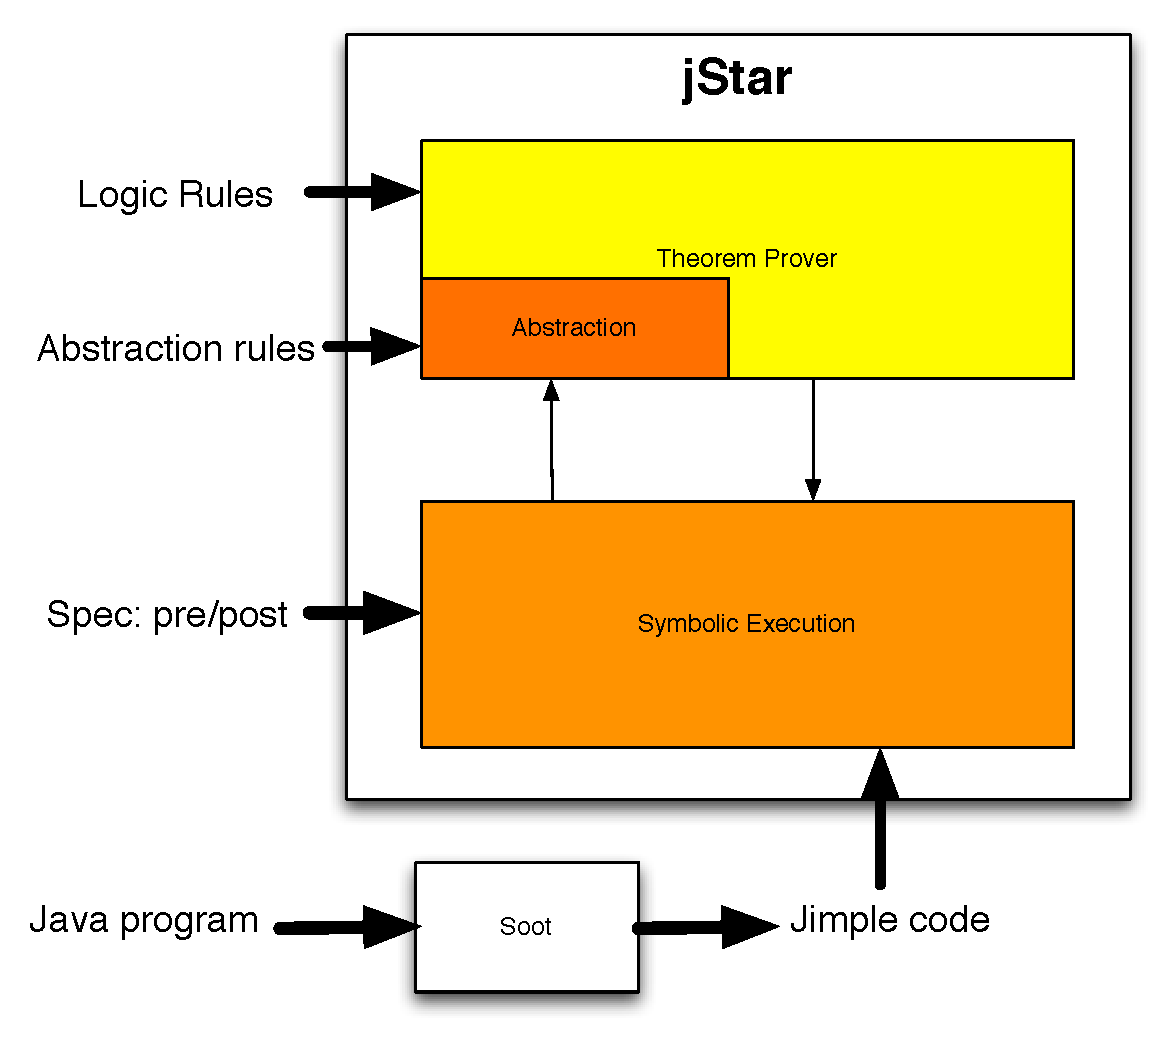
\includegraphics[width=2.9in]{architecture2}
  \caption[\jStarPlain\ architecture]{\jStar\ architecture}
  \label{fig:architecture}
\end{figure}
%
Other input files used by \jStar \ for the verification of a Java
program are:
\begin{description}
\item[Pre / post-condition specifications.]  This file
  specifies the
  pre and postconditions of the program's methods as well as the
  specifications of the methods called by it. 

  Details on pre / postcondition specifications are given in
  Section~\ref{sec:pre/post}.
\item[Logic rules.]  This file specifies the logical
  theory which is used by the theorem prover to decide entailment
  and other kinds of implications. The theory is specified by logical
  rules.  

  Details on logic rules are given in Section~\ref{sec:logic-rules}.
\item[Abstraction rules.]  This file defines the abstraction function
  used to ensure convergence in the fixed-point computation of
  loop invariants. The abstraction function is defined by means of
  abstraction rules that are an extension of the logical rules. 
  
  Details on abstraction rules are given in
  Section~\ref{sec:abstraction-rules}.~\jStarQED

\end{description}

\newcommand{\linkedlist}{\texttt{LinkedList.java}}



\subsection{Getting started}

To run  \jStar \ on a Java program we need first to compile it to the
Jimple intermediated language. To do this the Soot~\cite{vall99soot} package
must be installed and correctly working in your system. Consider the
\linkedlist \ program in Figure~\ref{tab:linkedlist}. Soot works on
bytecode, so we first compile it to produce the binary {\tt LinkedList.class}
with the command
\begin{verbatim}
 javac LinkedList.java
\end{verbatim}
We then run Soot to produce the Jimple version of our program:
\begin{verbatim}
java soot.Main LinkedList -f J -d .
\end{verbatim}
At this point the file {\tt LinkedList.jimple} should be in the
current directory. To run \jStar \ on the file {\tt LinkedList.jimple}
using the logical rules contained in {\tt LinkedList.logic}, the
abstraction rules in {\tt LinkedList.abs} and the specification rules
in {\tt LinkedList.specs} simply type the command
\begin{verbatim}
jstar -l LinkedList.logic -a LinkedList.abs -s LinkedList.specs   \
      -f LinkedList.jimple
\end{verbatim}
Here we are using the following \jStar \ command-line options:\footnote{For 
the complete list of options, run {\tt jstar -help}.} 
\begin{description}
\item[-l] specifies the file containing the {\em logic rules} used
    in this run of the verification.
\item[-a] specifies the file containing the {\em abstraction rules}.
\item[-s] specifies the file containing the pre/post specifications of the methods in the program.
\item[-f] specifies the Jimple translation of the program we want to
  verify.
\end{description}
\jStar \ will either report that all methods have been verified (meaning
that the \linkedlist \ meets the specifications defined in {\tt
  LinkedList.specs}), or report an error (indicating those methods
that could not be verified), or it will not terminate (indicating that the abstraction function
is not strong enough to ensure the termination of the invariant
computation).~\jStarQED

%
\begin{figure}[phtb]
  \centering
  \begin{tabular}{l@{\quad\;}|@{\quad}l}
    \begin{lstlisting}
class LinkedList
{
 private NodeLL head ;
 private NodeLL tail ;
 /* head == tail == null -> empty list */

 void create()
 {
  head=null;
  while (true) {
   NodeLL n = new NodeLL() ;
   n.next=head;
   head=n;
  }
 }
 
 void reverseList()
 {
  NodeLL f = null ; // finished part of list
  NodeLL r = head ; // rest of list to do
  NodeLL t = head ; // swap head and tail
  head = tail ;
  tail = t ;
  // Assert: Loop Invariant: list is split
  // between f and r, f being finished, r
  // needs to be processed.
  while ( r!=null )
  {
   t = r ; // to process t
   r = r.next ; // loop will terminate 
   t.next = f ; // put on head
   f = t ; // note: t has been used
  }
 }







${}$
\end{lstlisting}
&
\begin{lstlisting}   
 void insertAtHead( String newString )
 {
  NodeLL n = new NodeLL() ;
  n.content = newString ;
  n.next = head ;
  head = n ;
  if ( tail==null ) tail = head ;
 }

 void insertAtTail( String newString )
 {
  if ( head==null )
  {
   insertAtHead( newString ) ;
  }
  else
  {
   NodeLL n = new NodeLL() ;
   n.content = newString ;
   tail.next = n ;
   tail = n ;
  }
 }
 
 void printList()
 {
  NodeLL n = head ;
  while ( n!=null )
  {
   n = n.next ;
  }
 } 
} //end LinkedList class


class NodeLL
{
 String content ;
 NodeLL next ;
}
\end{lstlisting}
  \end{tabular}
  \caption{\linkedlist \ code.}
  \label{tab:linkedlist}
\end{figure}


\section{Pre/post condition specifications}
\label{sec:pre/post}
In this section we gives few practical notions and conventions needed
for writing specifications in \jStar. For a methodological introduction
on how to write specification in \jStar, and a collection of tricky
problems we refer the reader to~\cite{jstar}.

The program in Figure~\ref{tab:linkedlist} contains two classes
{\tt NodeLL}  representing a generic node for a linked list
and the \linkedlist \  combining nodes in 
singly-linked lists. To verify  \linkedlist \ in \jStar \ we
need to provide specification for:
\begin{itemize}
\item all
\linkedlist's methods;
\item the special method {\tt <init>()} introduced by Jimple
  (representing a constructor); and
\item  all the methods used by \linkedlist{}'s methods;
\end{itemize}
A specification is written as:
\begin{verbatim}
method_name(list parameter types): 
   { Precondition formula } 
   { Postcondition formula };
\end{verbatim}
%A formula is composed by two parts:
%\begin{verbatim}
%Pure part * Spatial Part
%\end{verbatim}
An example specification for the constructor of class {\tt NodeLL} is:
\begin{verbatim}
  static void <init>() : 
    {  } 
    {  field(@this:,<NodeLL: NodeLL next>,nil()) * 
       field(@this:,<NodeLL: java.lang.String content>,nil()) };
\end{verbatim}
%
The spec above tells us several syntactic conventions used by \jStar.
\begin{itemize}
\item An empty formula is a shorthand for $\true \wedge \emp$.
\item Following the Jimple notation, the Java special variable {\bf
    this} is written {\tt @this:}
\item The {\em points-to} predicate of separation logic is expressed by the
  predicate {\tt field(object, field name, content value)}. Hence 
  $o.f\psto v$ is written as {\tt field(o,f,v)}.
%\item Existentially quantified variables start with an underscore.
\item Field names must be written using their complete signature (as
  it is done by Jimple). Signatures in Jimple are  written {\tt <ClassName: TypeOfField NameOfField>}.
  Hence {\tt <NodeLL: java.lang.String content>} stands for the {\tt content} field of class {\tt NodeLL} 
  which has type {\tt java.lang.String}.
\end{itemize}
Intuitively the meaning of {\tt <init>}'s specification is:
\begin{quote}
\it
 ``Given an
empty heap the {\tt init} method returns an instance object of the {\tt node}
class expressed in terms of the {\tt field} predicate.''
\end{quote}
In separation
logic we would write this as the following Hoare triple:
\[
\{ true \wedge \emp \} \quad \texttt{<init>()} \quad \{ \this.next \psto \nil * \this.content \psto \nil \}
\]

\paragraph{Predicates definition.}
When writing specifications it is often useful to define predicates
which we will use inside specifications. This is similar to defining
objects which will be then used in the program. Predicate definitions
are of the form:
\begin{verbatim}
  define name_predicate(parameter_list) = Formula ;
\end{verbatim}
An alternative syntax accepted by \jStar \ replaces the equal sign by the keyword {\tt as}
\begin{verbatim}
  define name_predicate(parameter_list) as Formula ;
\end{verbatim}
Both syntaxes can be used interchangeably.
For example, for writing specifications for the \linkedlist \ class it
useful to define a predicate denoting a linked list. (Specifications of \linkedlist's class do nothing more than express
properties on linked lists.)
\begin{verbatim}
  define LL(x) =  
       field(x,<LinkedList: NodeLL tail>,_t) 
       * field(x,<LinkedList: NodeLL head>,_h) 
       * ( _t = nil() * _h = nil() 
        ||  _t!=nil() * lspe(_h,_t) * NodeLL(_t,nil())); 
\end{verbatim}
%
In separation logic this translates to:
\[\begin{array}{llll}
 LL(x) & = &  \exists t',h' \ldotp  &x.tail \psto t' * x.head \psto h' * {}
\\
& & & (t'=\nil * h'=\nil \wedge \emp ) 
\vee 
(t' \neq \nil \wedge \lseg(h',t') *NodeLL(t',\nil) )  
\end{array}
\]
This specification uses the predicate $NodeLL(a,b)$ denoting an instance of the class {\tt NodeLL}
and which can be written in separation logic as:
\[
  NodeLL(a,b) \;\; = \;\; a.{\it next} \psto b * a.{\it content} \psto c' 
\]
The formula
$LL(x)$ denotes either a list with only one element or a list with
the tail pointing to a node object. With the predicate $LL(x)$ we can
write easy specifications for the methods in {\tt LinkedList}.
All the specifications related to a class need do be enclosed between
a {\tt class} construct:
\begin{verbatim}
class LinkedList {
 ...
  void reverseList() : 
   {  LL$(@this:) } 
   {  LL$(@this:) };
 ...
}
\end{verbatim}
Here the \dollar \ sign is used to give a dual specification standing for both a dynamic and a static specification at the same time (see Section~\ref{sec:inheritance} for details on dynamic and static specifications and the use of \dollar).
\paragraph{On logical variables.}
Logical variables with names beginning with an underscore
are quantified variables.  Within a formula, a variable  {\tt \_x} is {\em existentially}
quantified (there is no need to write the quantifier explicitly). For example observe how {\tt \_t, \_h} in the example above correspond to $t'$ and $h'$ in the associated separation logic formula.

However, if a variable {\tt \_x}
occurs in both the pre and post-condition then it is {\em universally}
quantified (as in Hoare's logic). For example the specification:
\begin{verbatim}
{ Val$(@this:, {content=_X})} 
  get()
{ _X=$ret_var * Val$(@this:, {content=_X}) };
\end{verbatim}
corresponds to the Hoare triple:
\[
\forall \_X. \{ \,{\it Val}(\this,\_X) \,\} \;\; \text{\tt get()} \;\; \{ \_X={\it ret\_var} *  {\it Val}(\this, \_X)\}.
\]


\paragraph{On initialisation.} 
Every specification file must contain a specification for the {\tt <init>} method of the class {\tt java.lang.Object}. Normally this specification has an empty pre and postcondition:
\begin{verbatim}
class java.lang.Object 
{
static void <init>(): {  } {  };
}
\end{verbatim}
~\jStarQED

\subsection{Advanced specifications using inheritance}
\label{sec:inheritance}
We illustrate how inheritance can be dealt with in \jStar \ by mean of the following classes
\J~Cell~ and \J~Recell~:
\[
\begin{tabular}{@{}ll@{}}
\begin{lstlisting}
class Cell {
    int val;

    void set(int x) {
	val=x;
    }

    int get() {
	return val;
    }
}
\end{lstlisting}&\hspace{5em}
\begin{lstlisting}
class Recell extends Cell {
    int bak;

    void set(int x) {
	bak=super.get(); super.set(x);
    }

    int get() {
	return super.get();
    }
}
\end{lstlisting}
\end{tabular}
\]
The \J~Cell~ class has a \J~val~ field. This is updated by the
\J~set~ method and its value is returned by the \J~get~ method.  The
subclass \J~Recell~ has an additional field \J~bak~, which stores the
previous value the object held. 

To specify the \J~Cell~ class, we define a property \JS{Val} describing a \J~Cell~'s contents.  This is done with the following 
specification, defined inside the class \J~Cell~:
%
\begin{equation}
\label{eq:val}
\texttt{  define Val(x,content=y) as x.<Cell:int val> |-> y ;}
\end{equation}
%
This defines the property $\Val(x,\content y)$ to mean that the
field \JS{val} of object $x$ has contents $y$, \emph{provided} $x$ is
precisely of dynamic type \J~Cell~.  

% TODO: Not sure the following paragraph is correct! 

If $x$ is \emph{not} of this type,
then this definition does not constrain the meaning of the property. We call
$\Val$ an \emph{abstract predicate family}~\cite{Parkinson:popl05}. (Recall that $\Val$ is defined within \J~Cell~'s scope.)  One can
view this like a method definition: the definition of a method specifies its behaviour for a single class, not for all classes.

Definition (\ref{eq:val}) also (implicitly) defines another, related, property 
\[
\Val\J~@Cell~(x,\content y)
\]
$\Val\$\J~Cell~(x,\content y)$ refers to the definition of $\Val$  for type \J~Cell~. 
This property is visible (and therefore can be used) both inside \J~Cell~ and in any of \J~Cell~'s subclasses.
Since its scope covers  \J~Cell~ and its subclasses, the property $\Val\J~@Cell~(x,\content y)$
is independent of the actual dynamic type of \JS{x}. That is, it always asserts \JS{x}'s
\JS{val} field contains \JS{y} no matter where it is used (either \J~Cell~ or a subclass specifications)
and consequently no matter what \JS{x}'s type is (either \J~Cell~ or a subtype).  

We refer
to this second property as the \emph{internal property} as it
corresponds precisely to the body of the definition for a particular
class. Formally, we have the following two axioms:
\[
\begin{array}{@{}r@{\;}c@{\;}l@{}}
\begin{array}[b]{@{}l@{}}
\J~type~(x, \J~Cell~) \Longrightarrow \\
\mbox{}\qquad(\Val(x,\content y)
\end{array} & \iff & \Val\J~@Cell~(x,\content y))
\\[1em]
\Val\J~@Cell~(x,\content y) &\iff& x.val \mapsto y
\end{array}
\]
(Here, $\J~type~(x, \J~Cell~)$ means $x$ is precisely of dynamic type
\J~Cell~.)

The first axiom relates the internal property to the general property.  Note
that, this does not specify the meaning of $\Val(x,\content y)$ if $x$
is not of dynamic type \J~Cell~.  The second axiom specifies the internal
property.  This can be used to verify the class  \J~Cell~, but is not available
when verifying other classes.  That is, other classes (including
subclasses) must be independent of the specific internal definition of
the predicate (in the case of $\Val$, $ x.val \mapsto y$),
 but may mention the predicate abstractly (i.e., $\Val\J~@Cell~(x,\content y)$).



In \jStar \ we must provide two kinds of specification for each method: {\em static}
and {\em dynamic}~\cite{PB:popl08,chin08}.  The static specification gives a precise specification of the code's behaviour, while the
dynamic gives a more abstract view of how the method
behaves.  More specifically, the static specification is used for
\J~super~ and private calls and for verifying that it is sound to inherit a
method.  The dynamic specification is used for dynamic dispatch
and hence must be implemented by all subclasses (behavioural
subtyping~\cite{liskov94}).

We can specify the behaviour of the \J~get~ method by:
\begin{verbatim}
  int get() static:
    {@this:.val |-> _X }
    { _X=return * this.val|-> _X  };
  int get() dynamic:
    { Val$(@this:, {content= _X }) } 
    { _X= return * Val$(@this:, {content= _X }) };
\end{verbatim}
%
The first specification, the static specification, describes precisely
how the method updates the \JS{val} field.\footnote{In this case, the
  update of the method get() is the identity function.}  The
precondition $$\this.val \mapsto X$$ specifies that the \JS{val}
field of $\this$ has the value \JS{X} (a logical
variable). 
The postcondition $$X=\return * \this.val \mapsto X$$  specifies that the
field still has the same value, and that this value is returned,
$X=\return$.

The second specification, the dynamic specification, describes how the
method alters the more abstract \J~Val~ property, rather than the
concrete fields.  This enables subclasses to satisfy this
specification while changing the concrete behaviour, that is,
modifying different fields.

\begin{notation}
In \jStar \ only the {\tt static}
  qualifier needs to be explicitly stated. Without it 
  a method specification is assumed to be dynamic.
\end{notation}


The static specification we have given for \J~get~ is very concrete, since it is expressed in terms of the 
$val$ fields.  In order for subclasses of \JS~Cell~ 
 to use it, it must be restated more abstractly using the \JS{Val}\J~@Cell~ property.
\begin{verbatim}
 int get() static : 
  { Val$(this, {content=_X})} 
  { _X=return * Val$(@this:, {content=_X}) };
 \end{verbatim}
This specification describes for all subclasses precisely what the method body
does, but it does not reveal the fields that are actually modified.

As this pattern of specification is common, \jStar \ provides a shorthand,
which defines both the dynamic specification given above, and the second
static specification, with the single specification.
%
\begin{verbatim}
   int get() : 
     { Val$(this, {content=_X})} 
     { _X=return * Val$(@this:, {content=_X}) };
\end{verbatim}
%
A property postfixed by \J~@~ is interpreted by \jStar \ as the
standard property in the dynamic specification, that is without the
\J~@~, and as the internal property for the current class in the
static specification, in this case \JS{Val}\J~@Cell~.
%
Hence, both static and dynamic specifications for \J~set~  can be provided with only the following: 
\begin{verbatim}
   void set(int x) : 
     { Val$(this, {content=_})} 
     { Val$(this, {content=x}) };
\end{verbatim}
 The underscore stand for some value.
Remember that the behaviour of the constructor must be specified:
%
\begin{verbatim}
 void <init>() : { } { Val$(this,{content=_ }) };
\end{verbatim}
This specification stipulates that constructing an object gives the property
$$\exists \ex X.\Val(\this,\content{\ex X})$$ and that a call to a subclass's \J~super~
constructor results in the internal property
$$\exists \ex X.\Val\mbox{\$Cell}(\this,\content{\ex X})$$  This enables subclasses
to use this property without knowing its meaning.

We can now give the complete specification of the class \JS~Cell~:
\begin{verbatim}
class Cell {
  define Val(x,content=y) as x.<Cell: int val> |-> y ;

  void <init>() : { } { Val$(this,{content=_ }) };
  
  int get() : 
    { Val$(this, {content=_X})} 
    { _X=return * Val$(@this:, {content=_X}) };

  void set(int x) : 
    { Val$(this, {content=_})} 
    { Val$(this, {content=x}) };
}
\end{verbatim}

\paragraph{Recell.}
Now, let's consider \J~Recell~, a subclass of \J~Cell~.  First of all we must 
define what the \JS{Val} property means for the \J~Recell~ class.
%
% TODO: Don't understand width subtyping bit
\begin{verbatim}
 define Val(x,content=y;oldcon=z) as  Val$Cell(x, {content=y})  
                                      * x.<Recell: int bak>|-> z 
\end{verbatim}
%\begin{lstlisting}
%$\define  \Val(x,\contentOld y z ) = $
%    $\Val\mbox{\$Cell}(x,\content y) * x.bak \mapsto z$  ;
%\end{lstlisting}
If \JS{x} is of type \J~Recell~, this defines
$\Val(x,\contentOld y z)$ as the composition of the 
property associated to \JS{Val} from
the superclass \J~Cell~, and the new field \J~oldcon~ with value 
\JS{z}.  As we have defined the property with an additional labelled
parameter, \J~oldcon~, the system will also provide a meaning to the property
with only the \J~content~ parameter, for use when casting from \J~Cell~ to \J~Recell~.  In effect, we have width
subtyping on the labelled parameters, where missing parameters are
existentially quantified.  Hence, this defines $\Val(x,\content y)$
for the \J~Recell~ class as
\begin{verbatim}
Val(x, content=y) as Val$Cell(x,content= y ) 
                            * x.<Recell: int bak>|-> _z
\end{verbatim}
%
Importantly, by containing the \JS{Val}\J~@Cell~ property it allows the
\J~Recell~ to make super calls to the \J~Cell~'s methods, and also
inherit methods, as the precondition of \JS{Val}\J~@Cell~ can be
provided for the calls.
%
The specifications for \J~Recell~ is as follows:
%
\begin{verbatim}
class Recell {
  define Val(x,content=y;oldcon=z) as Val$Cell(x, {content=y}) 
                                      * x.<Recell: int bak>|-> z;

  void <init>() : { } { Val$(this, {content=_x; oldcon=_z}) };
  
  int get() : 
  { Val$(this, {content=_X; oldcon=_Y})} 
  { _X=return * Val$(this, {content=_X; oldcon=_Y}) };

  void set(int x) : 
  { Val$(@this:, {content=_X; oldcon=_})} 
  { Val$(@this:, {content=x; oldcon=_X}) };
}
\end{verbatim}
We must verify that these specifications are valid behavioural
subtypes, which follows from width subtyping of labelled
parameters.~\jStarQED


\section{Logic Rules}
\label{sec:logic-rules}
\jStar's  prover needs logic rules for deciding entailments. There are
two kinds of rule:
%
\begin{description}
\item[Pre-defined rules] are very general structural rules which need
  to be used with any kind of logic systems. These
  rules are hard-coded into the prover.
\item[User-defined rules] are problem-specific rules. They define a
  particular logic theory needed to solve the problem at hand. They
  must be provided by the user. Note that \jStar \ does not check that user-defined rules are 
  consistent. Therefore, the user should use special care in ensuring the soundness of rules.
\end{description} 
In this tutorial we focus on the second type of rules. Rules are introduced with
the syntactic construct {\tt rule}:
\begin{verbatim}
rule my_rule :
 | Conclusion-L |- Conclusion-R 
if 
 SubtFPre | Premise-L |- Premise-R
  \end{verbatim}
The keywords {\tt if} separates the conclusion from the premise.
Mathematically this syntax corresponds to
\[
\infer[\texttt{my\_rule}]
{ H_s \; \mid \; H_a *  \texttt{Conclusion-L}  \; \vdash \; H_g * \texttt{Conclusion-R} }
{ H_s * \texttt{SubtFPre} \; \mid \; H_a * \texttt{Premise-L } \; \vdash \; H_g * \texttt{Premise-R} 
%  \qquad   H_s * H_a \; \vdash \;  \texttt{SubFConc} 
} 
\] for some $H_s, H_a, H_g$. The rules work with sequents of the form
\[
\Sigma \; \mid \; F_1 \; \vdash \; F_2 
\]
We call $F_1$ the \emph{assumed formula}, $F_2$ the \emph{goal formula}, and $\Sigma$ the \emph{subtracted (spatial) formula}.  The semantics of a judgement is:
\[
F_1 *  \Sigma \Longrightarrow F_2 * \Sigma
\]
The subtracted formula $\Sigma$ is used to allow predicates to be
removed from both sides without losing information. 
Notice that rules are \emph{implicitly framed} | the semantics of the rule includes the contexts $H_s$, $H_a$ and $H_g$. This means rules can fire inside large context heaps. 
Hence the 
following example rule 
\begin{verbatim}
rule numeric_eq_right :
   | |- numeric_const(?x) = numeric_const(?y) 
if
   | |- ?x=?y
\end{verbatim}
encodes the implication:
\[
\infer[\texttt{rule numeric\_eq\_right}]{ H_s  \mid H_a \vdash \texttt{numeric\_const}(x) = \texttt{numeric\_const}(y) * H_g}{ H_s  \mid H_a \vdash x=y * H_g}
\]
Informally, this rule says: in any context $H_s, H_a, H_g$, if we want to prove the equality $\texttt{numeric\_const}(x) = \texttt{numeric\_const}(y)$ then we can prove the simpler fact $x=y$ in the same context.

\begin{notation}
 As specified in previous sections, existentially quantified variables
start with an underscore. Variables starting with a question mark as in the rule above are used for 
denoting any expressions (i.e., quantified variables, non-quantified variables, constant values, etc.). 
\end{notation}

\paragraph{Without clauses.}
Consider the following rule:
\begin{verbatim}
rule field_remove1:
| field(?x,?f,?y) |-  field(?x,?f,?t) 
without
  ?y!=?t 
if
  field(?x,?f,?y) | |- ?y=?t 
\end{verbatim}
This rule states that
if we have a field {\tt ?f} for the object {\tt ?x} in both the assumed and goal formula of an implication, to then move the 
 field to the subtracted formula, and to add the proof obligation that the values {\tt ?y} and {\tt ?t} are the same to the goal formula. 

The clause {\tt without} prevents the firing of the rule if the inequality {\tt ?y!=?t} is
present in the assumed formulae of the conclusion. In other words, it prevents the rule from firing when the assumed formula already says
that the fields have different values.  This clause is used to avoid the rule being applied
an infinite number of times.

We also allow the clause 
\begin{verbatim}
without  
   WO-L |- WO-R
\end{verbatim}
to allow the user to specify on which side the formula does not occur.

\paragraph{Contradictions.} 
A rule with an empty premise can be used to force the termination of the proof
search when we reached a contradictory statement.
%
For example consider the rule {\tt field\_nil\_contradiction}: 
\begin{verbatim}
rule field_nil_contradiction :
 | field(nil(),?f,?z) |-
if
\end{verbatim}
This rule fires when a field for {\tt nil()} is assumed to exist. Clearly, in that case
 we have found a contradiction, and {\tt field\_nil\_contradiction}  will stop the proof search.

\paragraph{With.}
We allow the user to specify a match to the obligation that may be
either in the already framed formula, or in the unmatched formula.
\begin{verbatim}
rule my_rule :
 With-L | Conclusion-L |- Conclusion-R 
if 
 SubtFPre | Premise-L |- Premise-R
  \end{verbatim}
Mathematically this syntax corresponds to
\[
\infer[\texttt{my\_rule}]
{ H_s \; \mid \; H_a *  \texttt{Conclusion-L}  \; \vdash \; H_g * \texttt{Conclusion-R} }
{ 
\begin{array}{c}
H_s * \texttt{SubtFPre} \; \mid \; H_a * \texttt{Premise-L } \; \vdash \; H_g * \texttt{Premise-R} 
  \\[0.2em]
   H_s * H_a \; \vdash \;  \texttt{With-L} 
\end{array}
} 
\] for some $H_s, H_a, H_g$. 

We can improve the previous rule by using the with formula.  
\begin{verbatim}
rule field_nil_contradiction :
 field(nil(),?f,?z) | |-
if
\end{verbatim}
This allows contradictions to be found in the already framed heap.  
\jStarQED


%For example the rule {\tt field\_not\_null} below
%states that it is always true that an object {\tt ?x} having a certain value in a field is an allocated object and 
%therefore it cannot be {\tt nil}. 
%\begin{verbatim}
%rule field_not_null :
%  field(?x,?f,?y) | |- ?x!=nil() 
%if
%  | |-
%\end{verbatim}


\section{Abstraction Rules}
\label{sec:abstraction-rules}
Abstraction rules are similar in syntax to logic rules, but they have a different purpose. They help the convergence of \jStar's computation when dealing with infinite domains. The idea is that an abstraction rule simplifies 
a formula so that it remains within a restricted class of heaps for which simplification is known to 
converge. The simplification is done by {\em rewriting}.  In general, simplification is
achieved by removing existentially quantified variables that do not appear
anywhere else in the heap. 

Abstraction rules are of the form:
\[
\infer[\mbox{(Abs Rule)}]{H* H' \leadsto H *H''}{ \mbox{condition}}
\]
Heap $H'$ is replaced by $H''$ if the condition holds.  $H''$ should be 
more abstract (simpler) than $H'$ since some unnecessary information is removed
(abstracted away). 
Heap $H$ is an arbitrary context preserved by the abstraction rule.

Given a set of abstraction rules, \jStar \  tries to use
any rules that can be applied to a heap. When no rules are applicable the resulting heap is maximally abstracted. 
Note that to ensure termination of this strategy, abstraction rules should be chosen so that each application strictly simplifies the heap.
Moreover, for soundness, the abstraction rules {\em must}
be true implications in separation logic. In other words, it must hold that:
\[
H*H' \Longrightarrow H*H''
\]
When designing abstraction rules
checking this implication gives an easy sanity condition for the 
soundness of the resulting fixed-point computation.

The syntax for abstraction rules uses the {\tt abstraction} construct and it is as follows:
\begin{verbatim}
abstraction my_abstraction_rule:
InitialFormula ~~>   AbstractFormula   
where  Condition
\end{verbatim}
The semantics of such a formula is:
\[
\infer[\texttt{my\_abstraction\_rule}]
{H* \texttt{InitialFormula} \;\; \leadsto \;\; H*\texttt{AbstractFormula} }{\texttt{Condition}}
\] 
%
The following is an abstraction rule for combining list predicates:
\begin{verbatim}
abstraction ls_ls:
 ls(?x,_x) * ls(_x,nil()) ~~>  ls(?x,nil())
where 
  _x notincontext;
  _x notin ?x
\end{verbatim}
Condition {\tt \_x notincontext} says that {\tt \_x} does not occur syntactically in the rest of the heap, i.e., in $H$. The condition {\tt \_x notin ?x} says that {\tt ?x} cannot be instantiated to {\tt \_x}. 
The rule would be written mathematically as:
\[
\infer[]
{H*ls(y,\_x)*ls(\_x,\nil) \;\; \leadsto \;\; H*ls(y,\nil)}
{\_x \notin Var(H) \cup \{ y \} }
\] 
%
This rule abstracts away from the useless quantified variable {\tt \_x}. It reduces the original heap involving two list-segment predicates to a simpler heap with only one such predicate.
\jStarQED

\paragraph{Acknowledgment.}
Distefano and Parkinson are both supported by Royal Academy of Engineering research fellowships. 
Dodds is supported by EPSRC.

\bibliographystyle{plain}
\bibliography{objects}

\appendix 
\section{Syntax of logic}

\begin{verbatim}
iop      ::=  +
          |   -
          |   <<
          |   >>
          |   >>>
          |   %
          |   /
          |   &


bop      ::=  <  
          |   >
          |   =
          |   !=
          |   <=
          |   >=

expression ::= (expression iop expression)
            |  field_signature
            |  integer_const
            |  - integer_const
              
variable ::=  name
          |   ? name
          |   _ name

formula  ::=  (formula)
          |   formula * formula
          |   formula || formula
          |   expression bop expression
          |   expression . expression |-> expression
          |   name ( expression , ... , expression ) 
          |   ! name ( expression , ... , expression ) 
          |   expression : name
          |   variable
          |   formula | formula                 [deprecated, lhs must be pure]
          |   False
\end{verbatim}

\section{A full Example}
In this section we report the specifications, logic, and abstraction rules to analyze the {\tt LinkedList} class
 reported in Figure~\ref{tab:linkedlist}.
\subsection{Specifications for the LinkedList class}
\begin{verbatim}
class java.lang.Object 
{
void <init>() static: { } { };
}

class NodeLL
{
  void <init>() static: 
    { } 
    { field(@this:,<NodeLL: NodeLL next>,nil()) * 
        field(@this:,<NodeLL: java.lang.String content>,nil())  };
}

class LinkedList
{
  define LL(x) =  
       field(x,<LinkedList: NodeLL tail>,_t) 
       * field(x,<LinkedList: NodeLL head>,_h) 
       * ( _t = nil() * _h = nil() 
        ||  _t!=nil() * lspe(_h,_t) * NodeLL(_t,nil())); 
       
  void <init>() : 
   { } 
   { field(@this:,<LinkedList: NodeLL tail>,nil()) 
       * field(@this:,<LinkedList: NodeLL head>,nil()) };

  void create() : 
   { field(@this:,<LinkedList: NodeLL tail>,nil()) 
       * field(@this:,<LinkedList: NodeLL head>,nil()) }
   { LL$(@this:) };

  void reverseList() : 
   { LL$(@this:) } 
   { LL$(@this:) };

  //This is called by insertAtTail with dynamic dispatch.
  void insertAtHead(java.lang.String) : 
   { LL$LinkedList(@this:) } 
   { LL$LinkedList(@this:) };

  void insertAtTail(java.lang.String) : 
   { LL$(@this:) } 
   { LL$(@this:) };

  void printList() : 
   { LL$(@this:) } 
   { LL$(@this:) };
}
\end{verbatim}

\subsection{Logic Rules for LinkedList}
\begin{verbatim}
import "../../src/prover/tests/field_logic";
import "../../src/prover/tests/boolean_logic";

/***************************************
 *  This file defines 
 *
 *  NodeLL
 *  ls
 *  lspe
 *
 ***************************************/
rule NodeLL_not_nil:
  NodeLL(nil(),?y) |  |- 
if

rule ls_not_nil:
  ls(nil(),?y) |  |- 
if

rule NodeLL_not_nil:
  lspe(nil(),?y) |  |- 
if
  | ?y=nil()  |- 

rule NodeLL_not_nil:
  NodeLL(?x,?y) |  |- ?x!=nil() 
if
  |  |- 

rule NodeLL_not_eq:
  NodeLL(?x,?y) * NodeLL(?x,?w) |  |- 
if

/*************************************
 * Rule for unpacking Nodell 
 *
 *  These rules could potentially cycle forever
 *  but due to their order cannot.
 *************************************/

//Unroll NodeLL if we are looking for its next field
rule field_remove1a:
  |   NodeLL(?x,?e1) |-  field(?x,"<NodeLL: NodeLL next>",?e2) 
if
    field(?x,"<NodeLL: NodeLL next>",?e1) 
|  field(?x,"<NodeLL: java.lang.String content>",_w)  |-  ?e1=?e2  

//Unroll NodeLL if we are looking for its content field
rule field_remove1b:
  |   NodeLL(?x,?e1) |-  field(?x,"<NodeLL: java.lang.String content>",?e2) 
if
     field(?x,"<NodeLL: java.lang.String content>",w) 
|   field(?x,"<NodeLL: NodeLL next>",?e1)   |-  w=?e2 

//Roll up a complete NodeLL if we have both fields.
rule field_remove2:
  |  field(?x,"<NodeLL: NodeLL next>",?e1) * 
      field(?x,"<NodeLL: java.lang.String content>",?z) |-  
if
  |  NodeLL(?x,?e1) |-   


/*************************************
 * Simple subtraction rules 
 *************************************/
rule ls_unroll_exists :
|  ls(?x,?y) |- | field(?x,?w,?Z)
if
|  NodeLL(?x,_fooz) * lspe(_fooz,?y)  |-  field(?x,?w,?Z)

rule ls_ls_match :
  ls(?z,?w) |  ls(?x,?y) |-  ls(?x,?z)
if
  ls(?x,?y) |  |-  lspe(?y,?z)

rule ls_NodeLL_match :
  NodeLL(?z,?w) |  ls(?x,?y) |-  ls(?x,?z)
if
  ls(?x,?y) |  |-  lspe(?y,?z)

rule ls_field_match :
  field(?z,?f,?w) | ls(?x,?y) |-  ls(?x,?z)
if
  ls(?x,?y) |  |- lspe(?y,?z)

rule nl_ls_match :
  ls(?z,?w) |  NodeLL(?x,?y) |-  ls(?x,?z)
if
  NodeLL(?x,?y) |  |-  lspe(?y,?z)

rule nl_NodeLL_match :
  NodeLL(?z,?w) |  NodeLL(?x,?y) |-  ls(?x,?z)
if
  NodeLL(?x,?y) |  |- lspe(?y,?z)

rule nl_field_match :
  field(?z,?f,?w) | NodeLL(?x,?y) |-  ls(?x,?z)
if
  ls(?x,?y) |  |-  lspe(?y,?z)

rule lspe_left :
  |  lspe(?x,?y) |-  
if
  |  ls(?x,?y) |-  ;
  | ?x=?y  |-  

rule lspe_right :
  |  |-  lspe(?x,?y) 
if
  |  |-  ls(?x,?y) 
or
  |  |- ?x=?y  

/*************************************
 * rules for contradictions 
 *************************************/
rule ls_field_contradiction1 :
ls(?x,?t) * field(?x,"<NodeLL: NodeLL next>",?z) |  |-  
if

rule ls_field_contradiction2 :
ls(?x,?t) * field(?x,"<NodeLL: java.lang.String content>",?z) |  |-  
if

rule ls_node_contradiction :
ls(?x,?t) * NodeLL(?x,?z) |  |-  
if

rule ls_ls_contr :
ls(?x,?t) * ls(?x,?z) |  |- 
if

rule ls_ls_contr :
 |  |- | ls(?x,?t) * ls(?x,?z)
if
 |  |- x!=x 
\end{verbatim}

\subsection{Abstraction Rules for LinkedList class}
\begin{verbatim}
//Roll up a complete NodeLL if we have both fields.
abstraction field_remove2:
   field(?x,"<NodeLL: NodeLL next>",?e1) * field(?x,"<NodeLL: java.lang.String content>",_y) 
~~>
   NodeLL(?x,?e1) 

abstraction type_remove :
  !type(?x,"NodeLL") * NodeLL(?x,?y)  ~~> NodeLL(?x,?y)  

/****************nil() rules******************/

abstraction nil_neq_remove_nodell :
  ?x != nil() * NodeLL(?x,?y) ~~> NodeLL(?x,?y) 

abstraction nil_neq_remove_field :
  ?x != nil() * field(?x,?f,?y) ~~> field(?x,?f,?y) 

abstraction nil_neq_remove_ls :
  ?x != nil() * ls(?x,?y) ~~>  ls(?x,?y) 

/*************** Junk Rules *******************/

abstraction garbage_garbage :
  Garbage * Garbage  ~~>  Garbage 


abstraction gb1_ls :
 ls(_x,?e) ~~>  Garbage 
where 
   _x notincontext 





abstraction gb1_ast :
  Ast(_x,?e) ~~>  
where 
   _x notincontext 


abstraction gb1_pto :
  NodeLL(_x,?e) ~~>  Garbage 
where 
   _x notincontext 


abstraction gb2_ls_ls:
  ls(_x,_y) * ls(_y,_x) ~~>  Garbage 
where 
   _x,_y notincontext


abstraction gb2_ls_pto:
  ls(_x,_y) * NodeLL(_y,_x) ~~>  Garbage 
where 
   _x,_y notincontext


abstraction gb2_pto_pto:
  NodeLL(_x,_y) * NodeLL(_y,_x) ~~>  Garbage 
where 
   _x,_y notincontext

/*************** End Junk Rules *******************/
/*************** Abs1 Rule *******************/
abstraction ls_ls:
 ls(?x,_x) * ls(_x,nil()) ~~> ls(?x,nil()) 
where 
  _x notincontext;
  _x notin ?x


abstraction ls_pto:
  ls(?x,_x) * NodeLL(_x,nil()) ~~>   ls(?x,nil()) 
where 
  _x notincontext;
  _x notin ?x




abstraction pto_ls:
  NodeLL(?x,_x) * ls(_x,nil()) ~~>  ls(?x,nil()) 
where 
  _x notincontext;
  _x notin ?x


abstraction pto_pto:
  NodeLL(?x,_x) * NodeLL(_x,nil()) ~~>  ls(?x,nil())
where 
  _x notincontext;
  _x notin ?x

/*************** End Abs1 Rule *******************/

/*************** Abs2 Rule *******************/
abstraction ls_ls_ls:
   ls(?x,_x) * ls(_x,?y) * ls(?y,?z) ~~>   ls(?x,?y) * ls(?y,?z) 
where 
  _x notincontext;
  _x notin ?x;
  _x notin ?y;
  _x notin ?z


abstraction ls_ls_pto:
   ls(?x,_x) * ls(_x,?y) * NodeLL(?y,?z) ~~>   ls(?x,?y) * NodeLL(?y,?z) 
where 
  _x notincontext;
  _x notin ?x;
  _x notin ?y;
  _x notin ?z


abstraction ls_pto_ls:
   ls(?x,_x) * NodeLL(_x,?y) * ls(?y,?z) ~~>   ls(?x,?y) * ls(?y,?z)
where 
    _x notincontext;
  _x notin ?x;
  _x notin ?y;
  _x notin ?z






abstraction ls_pto_pto:
   ls(?x,_x) * NodeLL(_x,?y) * NodeLL(?y,?z) ~~>   ls(?x,?y) * NodeLL(?y,?z)
where 
  _x notincontext;
  _x notin ?x;
  _x notin ?y;
  _x notin ?z


abstraction pto_ls_ls:
   NodeLL(?x,_x) * ls(_x,?y) * ls(?y,?z) ~~>   ls(?x,?y)  * ls(?y,?z) 
where 
  _x notincontext;
  _x notin ?x;
  _x notin ?y;
  _x notin ?z


abstraction pto_ls_pto:
   NodeLL(?x,_x) * ls(_x,?y) * NodeLL(?y,?z) ~~>   ls(?x,?y)  * NodeLL(?y,?z)
where 
  _x notincontext;
  _x notin ?x;
  _x notin ?y;
  _x notin ?z


abstraction pto_pto_ls:
   NodeLL(?x,_x) * NodeLL(_x,?y) * ls(?y,?z) ~~>   ls(?x,?y) * ls(?y,?z) 
where 
  _x notincontext;
  _x notin ?x;
  _x notin ?y;
  _x notin ?z


abstraction pto_pto_pto:
   NodeLL(?x,_x) * NodeLL(_x,?y) * NodeLL(?y,?z) ~~>   ls(?x,?y) * NodeLL(?y,?z) 
where 
  _x notincontext;
  _x notin ?x;
  _x notin ?y;
  _x notin ?z
\end{verbatim}
\end{document}